\documentclass[%
 reprint,
%superscriptaddress,
%groupedaddress,
%unsortedaddress,
%runinaddress,
%frontmatterverbose, 
%preprint,
%showpacs,preprintnumbers,
%nofootinbib,
%nobibnotes,
%bibnotes,
 amsmath,amssymb,
 aps,
%pra,
%prb,
%rmp,
%prstab,
%prstper,
%floatfix,
]{revtex4-1}

\usepackage{graphicx}% Include figure files
\usepackage{dcolumn}% Align table columns on decimal point
\usepackage{bm}% bold math
%\usepackage{hyperref}% add hypertext capabilities
%\usepackage[mathlines]{lineno}% Enable numbering of text and display math
%\linenumbers\relax % Commence numbering lines

%\usepackage[showframe,%Uncomment any one of the following lines to test 
%%scale=0.7, marginratio={1:1, 2:3}, ignoreall,% default settings
%%text={7in,10in},centering,
%%margin=1.5in,
%%total={6.5in,8.75in}, top=1.2in, left=0.9in, includefoot,
%%height=10in,a5paper,hmargin={3cm,0.8in},
%]{geometry}

\usepackage{cmap} % Поиск в PDF
\usepackage[T2A]{fontenc} % Кодировка
\usepackage[utf8]{inputenc} % Кодировка исходного текста
\usepackage[english, russian]{babel} % Локализация и переносы
\frenchspacing % Более тонкая настройка пробелов 
\usepackage{multirow}
\usepackage[warn]{mathtext}
\usepackage{amssymb}
\usepackage{ dsfont }
\usepackage{ textcomp }
\usepackage{ mathrsfs }

% Переопределение англоязычного начертания каппа, фи и эпсилон, 
% а также знаков сравнения
\renewcommand{\epsilon}{\ensuremath{\varepsilon}}
\renewcommand{\phi}{\ensuremath{\varphi}} 
\renewcommand{\kappa}{\ensuremath{\varkappa}}
\renewcommand{\le}{\ensuremath{\leslant}}
\renewcommand{\leq}{\ensuremath{\leqslant}}
\renewcommand{\ge}{\ensuremath{\geslant}}
\renewcommand{\geq}{\ensuremath{\geqslant}}
\renewcommand{\emptyset}{\ensuremath{\varnothing}}

\usepackage{textcomp} 
\usepackage{indentfirst} % Красная строка
\usepackage{amsmath} % Текст в формулах
\usepackage{graphicx} % Графика
\DeclareGraphicsExtensions{.pdf,.png,.jpg}
\usepackage{pgfplots}
\pgfplotsset{compat=1.13}

%\usepackage{times}

\begin{document}

\title{Определение энергии $\alpha$-частиц по величине их пробега в воздухе}
\thanks{4.1}

\author{Иван Едигарьев}
\affiliation{
 Московский Физико-Технический Институт\\
 Факультет Общей и Прикладной Физики, 526т\\
}
%\date{\today}

\begin{abstract}
Измеряется пробег $\alpha$-частиц в воздухе двумя способами: с помощью торцевого счетчика Гейгера и сцинтилляционного счетчика, - по полученным величинам определяется энергия частиц.

\end{abstract}

\pacs{Valid PACS appear here}

\maketitle

\begin{enumerate}

\item 
\textbf{Исследование пробега $\alpha$-частиц с помощью счетчика Гейгера}\\
Включим установку и проверим ее функционирование. Дадим ей прогреться. Проведем предварительные измерения для определения вида зависимости количества частиц от расстояния до счетчика Гейгера.

Снимем зависимость скорости счета N за 100 секунда от расстояния между источником и счетчиком.

\begin{figure}[h]
\center{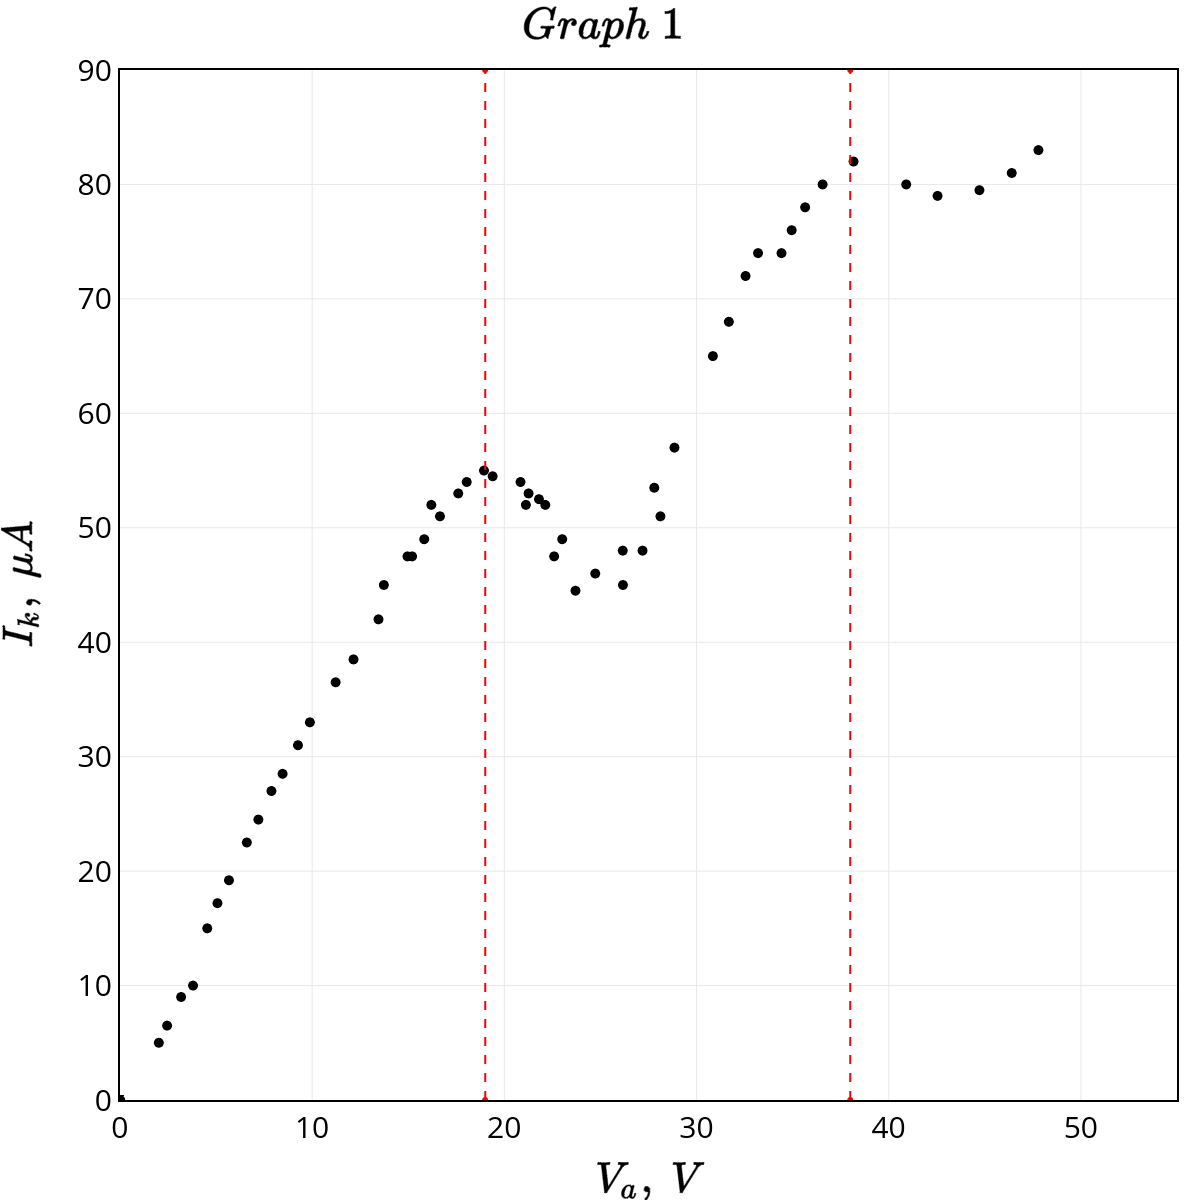
\includegraphics[scale=0.17]{my_plot1.png}}
\end{figure}

Построим график зависимости $N=N(x)$, и определим по нему средний и экстраполированный пробег $\alpha$-частиц
\begin{gather*}
R_{\text{э}} = (0.9 \pm 0.2 + 1.0)~cm = (2.1 \pm 0.2)\cdot10^{-3}~g/cm^2\\
R_{\text{ср}} = (0.7 \pm 0.2 + 1.0)~cm = (1.8 \pm 0.2)\cdot10^{-3}~g/cm^2.
\end{gather*}
\item
\textbf{Определение пробега $\alpha$-частиц с помощью сцинтилляционного счетчика}\\
Включим установку и проверим ее функционирование. Дадим ей прогреться. Проведем контрольные опыты и предварительные измерения.

Изменяя давление в камере, измерим количество частиц, фиксируемых счетчиком за 100 секунд.

\begin{figure}[h]
\center{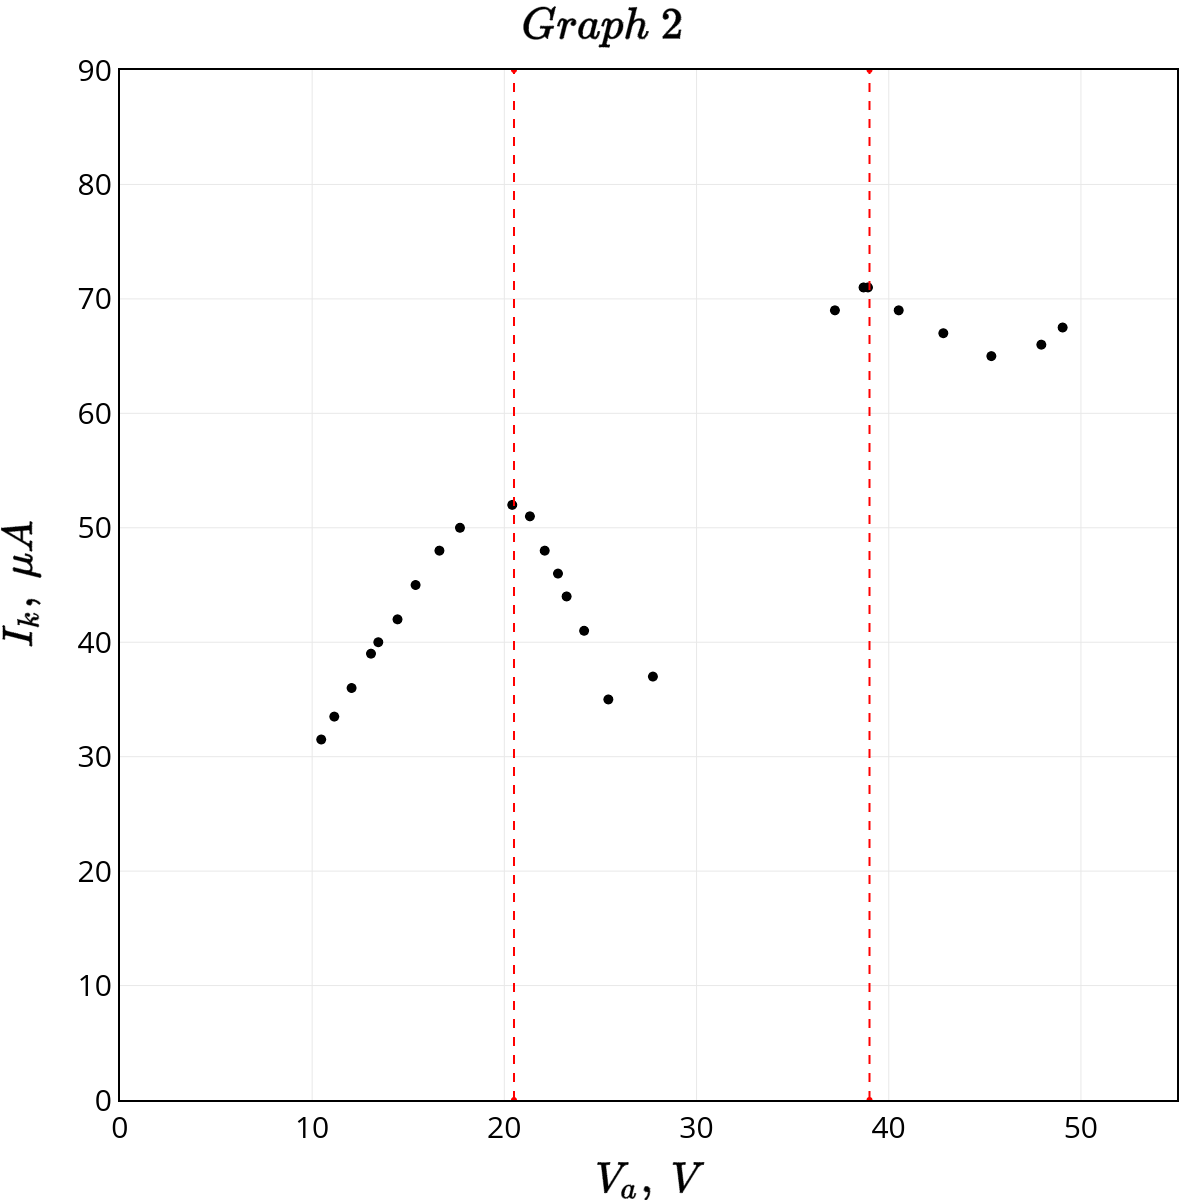
\includegraphics[scale=0.17]{my_plot2.png}}
\end{figure}

Построим график зависимости $N=N(P)$, и определим по нему средний и экстраполированный пробег $\alpha$-частиц, а так же их энергию
\begin{gather*}
R_{\text{ср}}^{1, 1}((220 \pm 5)~torr,~300K) = 9~cm \Rightarrow\\
R_{\text{ср}}^{0, 0}(P_0, T_0) = \frac{T_0}{T_1} \frac{P_1}{P_0}R_{\text{ср}}^{1, 1} = (2.5 \pm 0.1)~cm =\\
= (3.0 \pm 0.1)\cdot10^{-3}~g/cm^2.\\
R_{\text{э}}^{2, 1}((310 \pm 5)~torr,~300K) = 9~cm \Rightarrow\\
R_{\text{э}}^{0, 0}(P_0, T_0) = \frac{T_0}{T_1} \frac{P_2}{P_0}R_{\text{ср}}^{2, 1} = (3.5 \pm 0.1)~cm =\\
= (4.3\pm0.1)\cdot10^{-3}~g/cm^2.\\
E_{\text{ср}} = \left( \frac{R_{\text{ср}}}{0.32} \right)^{2/3} = (3.9 \pm 0.2)~MeV, \\
E_{\text{э}} = \left( \frac{R_{\text{э}}}{0.32} \right)^{2/3} = (4.9 \pm 0.2)~MeV.
\end{gather*}
% Из сравнения результатов определим толщину слюды закрывающей окно торцевого счётчика.

% Считая, что эффективность счёта $\alpha$-частиц равна 100$\%$, оценим по известному периоду полураспада количество вещества в препарате. 

\item
\textbf{Исследование пробега $\alpha$-частиц с помощью ионизационной камеры}\\
Включим установку и проверим ее функционирование. Дадим ей прогреться. Проведем контрольные опыты и предварительные измерения. 
% Изменяя давление в камере, измерим ионизационный ток в камере.
Построим график зависимости $I=I(P)$, и определим по нему экстраполированный пробег $\alpha$-частиц, а так же их энергию

\begin{gather*}
R_{\text{э}}^{3, 1}((510 \pm 5)~torr,~300K) = 5~cm \Rightarrow\\
R_{\text{э}}^{0, 0}(P_0, T_0) = \frac{T_0}{T_1} \frac{P_3}{P_0}R_{\text{ср}}^{3, 1} = (3.2 \pm 0.1)~cm =\\
= (3.9\pm0.1)\cdot10^{-3}~g/cm^2.\\
E_{\text{э}} = \left( \frac{R_{\text{э}}}{0.32} \right)^{2/3} = (4.6 \pm 0.2)~MeV.
\end{gather*}

\begin{figure}[h]
\center{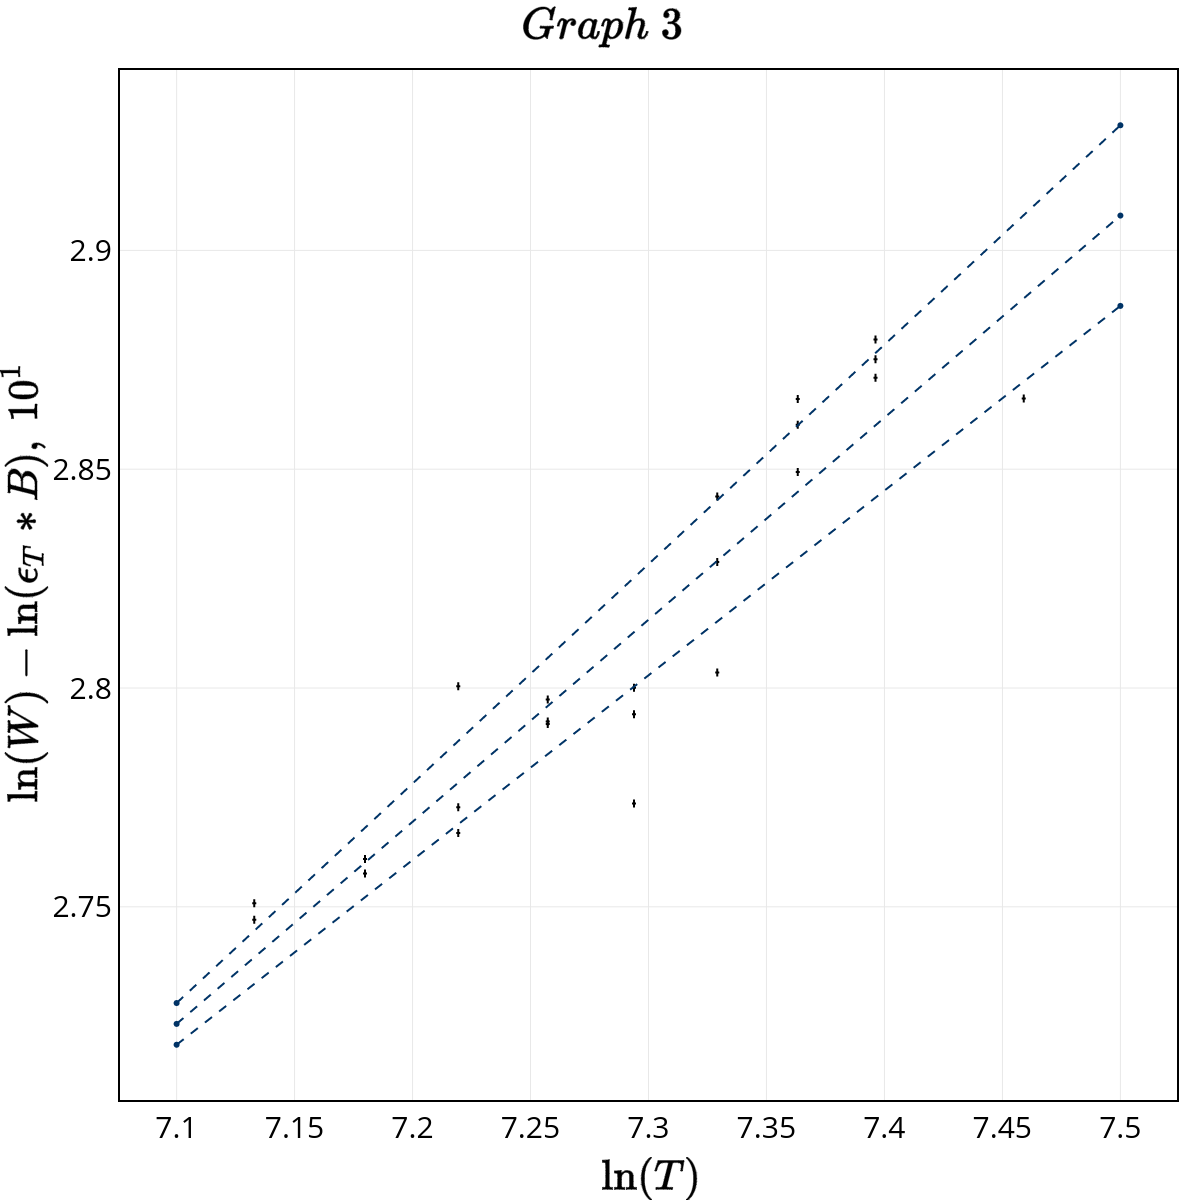
\includegraphics[scale=0.17]{my_plot3.png}}
\end{figure}

Сравним значение энергии с табличным
\begin{gather*}
E_{\text{table}} = 5.15~MeV.
\end{gather*}

\end{enumerate}

\end{document}